\section[二期：离散 Token 预测与音乐生成]{二期扩展：从判别式分类到离散 Token 预测与音乐生成}\label{sec:phase2}

一期的全部实验都是判别式的：给定 5 秒音频，输出 10 个（或 8 个）流派标签之一。
一个自然的问题是——同一个系统能否回答"接下来会发生什么"？本章把任务从"分类"
推进到"预测"与"生成"，并严格区分两类结果：一是对\textbf{真实未来}的 Token 级预测，
二是在\textbf{前缀条件}下的音乐续写。前者可以用交叉熵和 Top-1 精确度量，后者只能部分
度量、必须结合试听，二者的评价口径不能混用。

\subsection{任务定义与动机}\label{sec:p2motivation}

一期与二期的差别可以写成两个不同的条件分布：

\begin{itemize}
  \item 分类：$p(y \mid \mathbf{x}_{1:T})$，$y$ 为流派标签，$\mathbf{x}$ 为 5 秒音频；
  \item 预测：$p(\mathbf{c}_{T+1:T+K} \mid \mathbf{c}_{1:T})$，$\mathbf{c}$ 为离散音频 Token；
  \item 生成：$p(\mathbf{x}_{T+1:T+K'} \mid \mathbf{x}_{1:T}, \text{text})$，输出是可播放的波形。
\end{itemize}

选择 Token 而不是波形，有两个工程理由。第一，离散 Token 把"预测音频"变成了
"预测离散符号"，可以直接复用语言模型的训练与评价方法（交叉熵、Top-$k$、自回归
roll-out），不需要设计波形回归损失或对抗训练。第二，它把"模型是否学到了音乐的
时间结构"与"声码器是否好听"解耦——若 Token 预测很差，问题就不在解码器。

本章的实验设计刻意保持"可控"：Token 预测部分只用 5 秒前缀预测 1 秒真实未来，
模型是自己训练的小网络，不调用任何生成大模型；生成部分才引入预训练的
MusicGen-small，并先验证原始模型能跑通、再讨论轻量适配。

\subsection{离散音频 Token：EnCodec 32 kHz}\label{sec:encodec}

编码器选用 \texttt{facebook/encodec\_32khz}，即 MusicGen 使用的同款配置。它把
32 kHz 单声道波形经卷积编码器与残差向量量化（RVQ）压成 4 个码本、每码本 2048 个
词条的离散序列，帧率 50 Hz，目标带宽 2.2 kbps。表~\ref{tab:encodec} 给出实测规格。

\begin{table}[H]
\centering\small
\caption{EnCodec 32 kHz 的实测规格（6 秒窗口）。}\label{tab:encodec}
\begin{tabular}{ll}
\toprule
项目 & 实测值\\
\midrule
检查点 / 参数量 & \texttt{facebook/encodec\_32khz} / 56.9\,M（约 228\,MB）\\
采样率 / 声道 & 32\,000\,Hz / 单声道\\
码本数与词表 & 4 个码本 $\times$ 2\,048\\
帧率 & 50\,Hz（1\,s $=$ 50 帧，6\,s $=$ 300 帧）\\
6 秒窗口 Token 量 & $4 \times 300 = 1\,200$\\
编码输出形状 & \texttt{audio\_codes} $=(n_{\text{frames}},\,B,\,4,\,T)$，本实验 $n_{\text{frames}}=1$\\
解码回波形 & \texttt{audio\_values} $=(B,\,T\times 640)$，48\,k 采样点 $=$ 6\,s\\
编码吞吐（8 卡批次） & 8$\times$6\,s 约 0.34\,s（fp32，RTX 4060）\\
\bottomrule
\end{tabular}
\end{table}

有一个容易被忽略的兼容性细节：\texttt{transformers} 的编码输出第一维是
"分段数"而不是批大小，若直接把 \texttt{audio\_codes[:, 0]} 当作批维，
批内除第一段以外的样本会被静默丢弃——本项目在第一次全量编码时就踩了这个坑
（每 512 个窗口只写入 1 行 Token），发现后修正并重跑。这类"形状对得上、语义却错"
的 bug 不会报错，只会让数据静默变少，因此下表的所有统计都同时核对了 Token 行数与
窗口行数。

\subsection{数据窗口与泄漏控制}\label{sec:p2data}

数据沿用 FMA-small 与一期按艺术家分离的划分（5\,596 / 1\,199 / 1\,199）。
每首曲目在其内部取 2 个不重叠的 6 秒窗口：前 5 秒作为前缀（250 帧），
后 1 秒作为预测目标（50 帧）。窗口继承曲目所属划分，因此\textbf{同一首歌的窗口不会同时出现在训练集与测试集}——这正是分类实验里那条"按艺术家划分"的约束在预测任务
上的对应物。最终得到 \TokNTrain{} 个训练窗口、测试集 \TokNTest{} 个窗口
（\TokNTracks{} 首曲目），Token 缓存以 shard 形式落盘，编码中断可从断点续跑。

\subsection{预测模型}\label{sec:p2models}

所有模型都做同一件事：给定前 $t$ 帧的 4 个码本，预测第 $t+1$ 帧的 4 个码本。
四条流共享一个主干，输出 4 个独立分类头（MusicGen 式的并行码本预测），
这样可以避免自回归解码时四条流不同步的问题。

\begin{table}[H]
\centering\small
\caption{Token 预测模型与基线。}\label{tab:tokenmodels}
\begin{tabular}{l p{7.6cm} r}
\toprule
模型 & 结构 & 参数量\\
\midrule
Persistence & 重复前缀最后一帧，不做任何学习 & 0\\
频率先验 & 训练集各码本最高频 Token & 0\\
Bigram & $p(t\mid t-1)$ 加 0.5 平滑，回落至 unigram & 0\\
LSTM & 4 个 Embedding 求和 $+$ 位置编码 $+$ 2 层 LSTM(256) $+$ 4 头 & 5.3\,M\\
Transformer & 4 个 Embedding 求和 $+$ 位置编码 $+$ 4 层因果注意力($d=192$, 4 头) $+$ 4 头 & \TokTfParams\\
\bottomrule
\end{tabular}
\end{table}

选择"并行码本"而不是"逐码本级联"，代价是模型必须同时刻画四条残差流之间的
相关性；收益是推理时一次前向就能得到完整的一帧，且解码器可以直接消费。
单码本（只预测码本 0）是更便宜的简化，但它\textbf{无法单独解码}，因此本文不做单码本
主结果，只把它作为反面对照写进局限性。

\subsection{训练与评价口径}\label{sec:p2train}

训练目标是四个码本的平均交叉熵。优化器 AdamW（学习率 $3\times10^{-4}$，权重衰减
0.01），余弦退火，梯度裁剪 1.0，batch 64，早停耐心 3 个 epoch，按验证集 NLL 选择
最优权重；每个模型跑 3 个随机种子（42/123/2024），测试集只在最后评估一次。

评价分两种口径，必须同时报告：

\begin{itemize}
  \item \textbf{teacher-forced}：第 $t$ 步喂入真实的历史 Token，度量"给定正确历史时
        分布有多准"，即标准的 NLL / Top-1；
  \item \textbf{free-running}：模型把自己的预测喂回下一步，度量"真正生成时"的准确率。
        两者差距越大，说明误差累积越严重。
\end{itemize}

\subsection{Token 预测结果}\label{sec:p2results}

\begin{table}[H]
\centering\small
\caption{Token 预测结果（FMA-small 测试集，5 s 前缀 → 1 s 目标）。神经网络为 3 个种子的均值 $\pm$ 标准差，基线为确定性预测。}
\label{tab:token}
\begin{tabular}{lccccc}
\toprule
模型 & 参数量 & NLL & Teacher Top-1 & Free Top-1 & 码本 0 Top-1\\
\midrule
Persistence & -- & -- & 0.016 & 0.016 & 0.024\\
频率先验 & -- & -- & 0.012 & 0.012 & 0.009\\
Bigram & -- & -- & 0.017 & 0.017 & 0.024\\
LSTM & 5.3M & 6.821 & 0.020$\pm$0.000 & 0.016$\pm$0.000 & 0.016\\
Transformer & 5.0M & 6.725 & 0.024$\pm$0.000 & 0.019$\pm$0.000 & 0.023\\
\bottomrule
\end{tabular}
\end{table}


\begin{figure}[H]
\centering
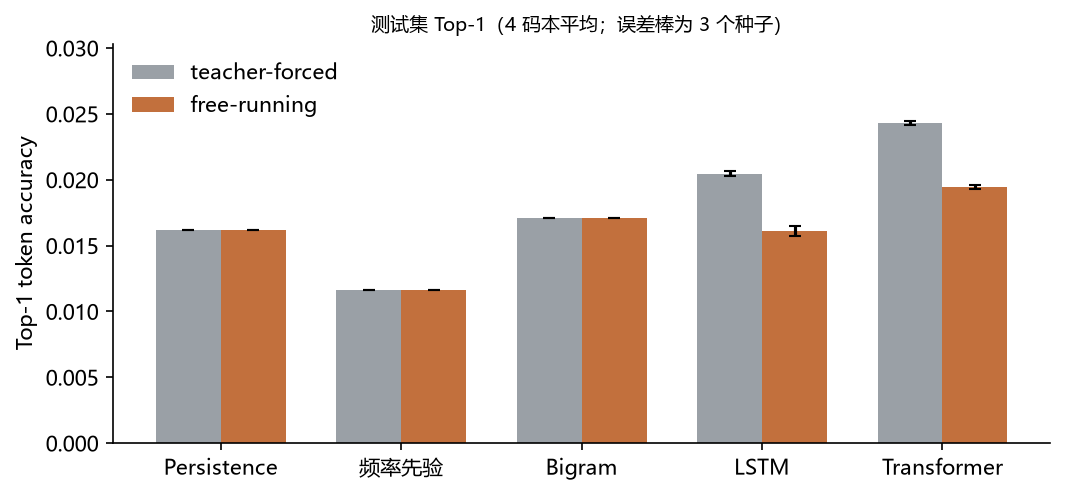
\includegraphics[width=\textwidth]{token_top1.png}
\caption{测试集 Top-1（4 码本平均）。灰色为 teacher-forced，橙色为 free-running，
误差棒为 3 个种子的标准差。}\label{fig:tokentop1}
\end{figure}

\begin{figure}[H]
\centering
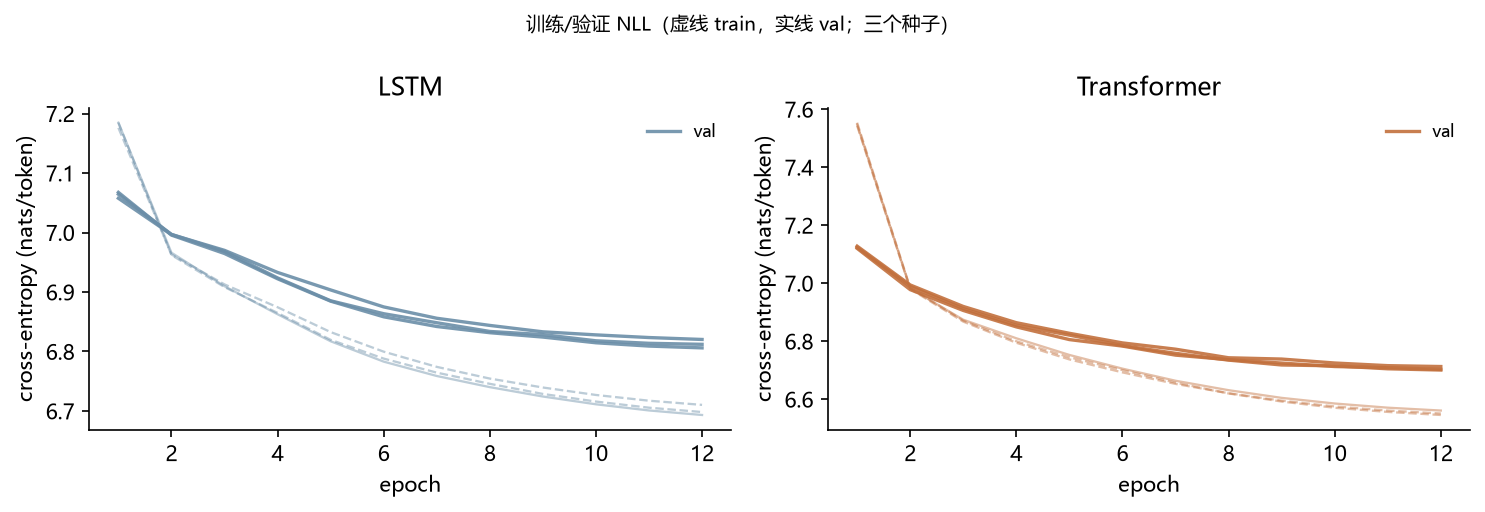
\includegraphics[width=0.92\textwidth]{token_curves.png}
\caption{训练与验证 NLL 曲线：三个种子的验证曲线几乎重合，说明小模型在固定数据上
训练稳定。}\label{fig:tokencurves}
\end{figure}

\begin{figure}[H]
\centering
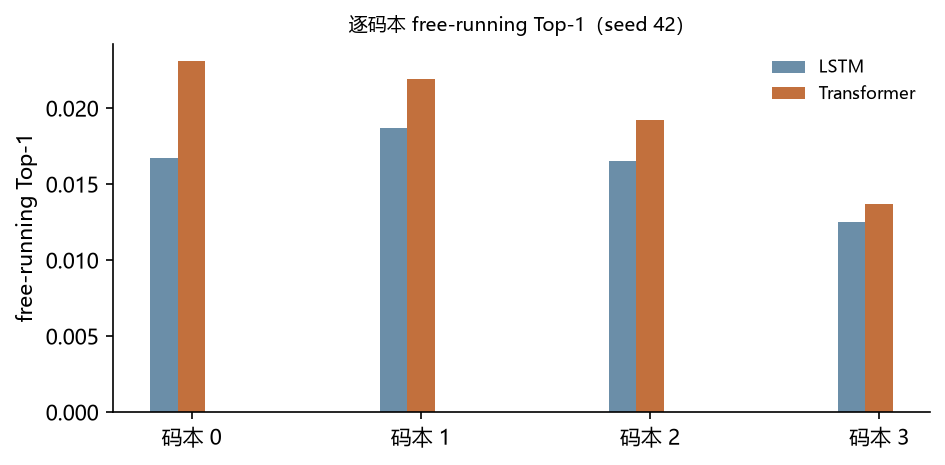
\includegraphics[width=0.78\textwidth]{token_per_codebook.png}
\caption{逐码本 free-running Top-1（seed 42）。码本 0 最容易，靠后的残差码本更难，
与 RVQ 的残差结构一致。}\label{fig:tokencb}
\end{figure}

四点观察：

\begin{enumerate}
  \item \textbf{学习信号真实存在，但绝对水平很低。}随机猜的 Top-1 是 $1/2048=0.049\%$；
        Transformer 的 free-running Top-1 为 \TokTransformerFree{}，约为随机的 40 倍，
        比最好的统计基线 Bigram（\TokBigramFree{}）高 0.24 个百分点（相对提升约 14\%）；
        NLL 从均匀分布的值 $\ln 2048 = 7.62$ 降到 \TokTransformerNll{}。
  \item \textbf{误差累积是主要损失来源。}Transformer 的 teacher-forced Top-1 为
        \TokTfTeacher{}，free-running 掉到 \TokTransformerFree{}；LSTM 也从
        \TokLstmFree{} 的教师强制口径下降。一旦让模型吃自己的预测，错误逐步放大——
        这正是自回归模型在长 horizon 上的典型退化。
  \item \textbf{LSTM 没有赢过 n-gram。}LSTM 的 free-running Top-1（\TokLstmFree{}）甚至
        略低于 Bigram（\TokBigramFree{}）。原因不是"没训练好"（其 NLL 明显低于 Bigram），
        而是循环状态在自回归回灌下更不稳定；小 Transformer 的因果注意力在本任务上更有效。
  \item \textbf{第一码本靠"重复"就够，增益来自残差码本。}Persistence 在码本 0 上能拿到
        2.43\%，与 Transformer 的 2.31\% 相当；但四码本平均时 Persistence 只有
        \TokPersistenceFree{}。这说明码本 0 高度局部平滑（音乐瞬时音色变化慢），
        神经模型的收益主要来自后三个残差码本。
\end{enumerate}

\subsection{把 Token 解码回音频}\label{sec:p2decode}

预测得准不等于"能听"。由于本实验预测全部 4 个码本，可以直接交给 EnCodec 解码：

\begin{enumerate}
  \item 用模型自回归生成 50 帧 $\times$ 4 码本；
  \item 送入 EnCodec 解码器得到 1 秒波形；
  \item 与原曲真实后 1 秒做 Log-Mel 对照，并保存 wav 供试听。
\end{enumerate}

\begin{table}[H]
\centering\small
\caption{预测 Token 解码回音频后与真实后 1 秒的对照（Log-Mel RMSE，越小越接近）。}
\label{tab:tokensamples}
\begin{tabular}{llcc}
\toprule
曲目 & 流派 & Log-Mel RMSE & 试听\\
\midrule
001482 & Electronic & 14.43 & \texttt{001482\_Electronic\_pred.wav}\\
000995 & Experimental & 7.74 & \texttt{000995\_Experimental\_pred.wav}\\
000814 & Folk & 13.73 & \texttt{000814\_Folk\_pred.wav}\\
007481 & Hip-Hop & 18.01 & \texttt{007481\_Hip-Hop\_pred.wav}\\
014568 & Instrumental & 21.13 & \texttt{014568\_Instrumental\_pred.wav}\\
000704 & International & 17.05 & \texttt{000704\_International\_pred.wav}\\
000010 & Pop & 13.12 & \texttt{000010\_Pop\_pred.wav}\\
000182 & Rock & 15.33 & \texttt{000182\_Rock\_pred.wav}\\
\bottomrule
\end{tabular}
\end{table}


\begin{figure}[H]
\centering
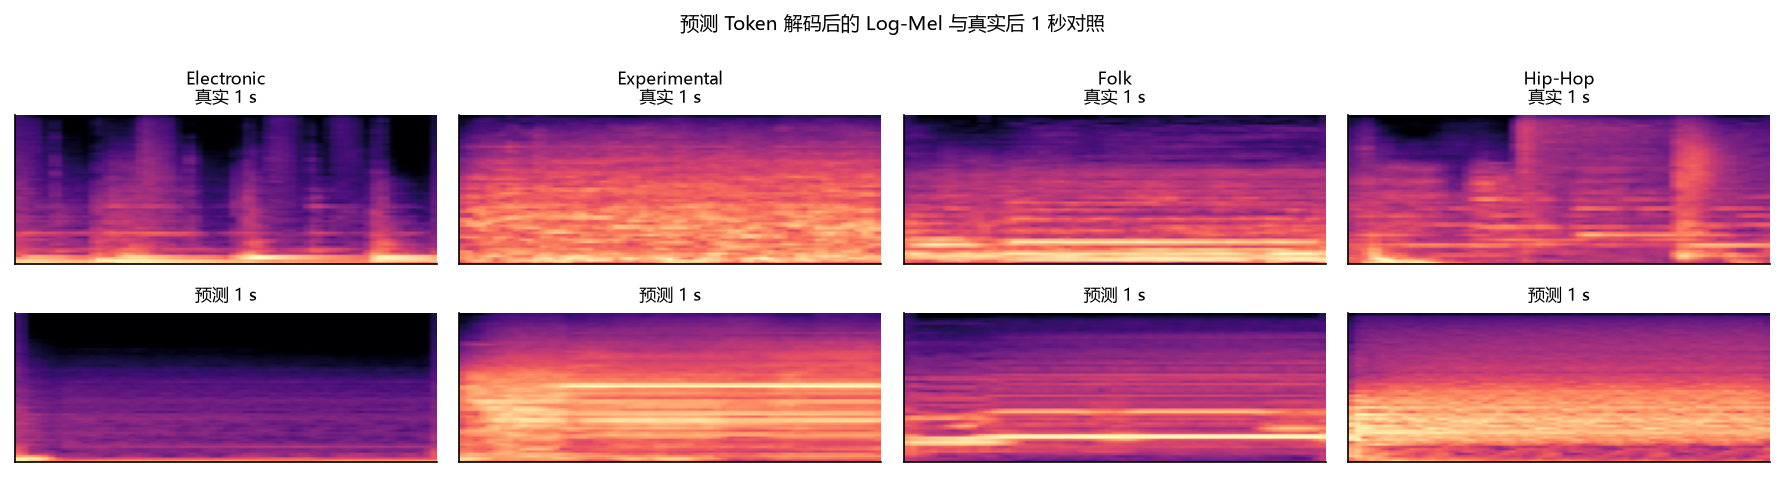
\includegraphics[width=\textwidth]{token_decode.png}
\caption{预测 Token 解码后的 Log-Mel（下）与真实后 1 秒（上）。整体能量包络接近，
但高频细节明显不同——这正是 Top-1 准确率无法表达的差异。}\label{fig:tokendecode}
\end{figure}

必须说明的局限：即便 4 个码本全部由模型预测，1 秒的预测也只能"猜"出下一个瞬间的
音色与节奏，无法生成有结构的乐句。它验证的是"模型是否学到了局部动态"，而不是
"能否续写一首歌"。后者属于下一节的生成任务。

\subsection{MusicGen-small 的前缀续写}\label{sec:musicgen}

生成阶段使用 \texttt{facebook/musicgen-small}（文本条件自回归 Transformer，
4 码本、50\,Hz、与上一节同一套 EnCodec Token）。官方 \texttt{audiocraft} 实现支持
"音频续写"开关，但它对本环境的 PyTorch 版本有强约束；为不破坏一期环境，本文改用
\texttt{transformers} 中同一个模型的解码器，按官方文档的方式构造延续：

\begin{enumerate}
  \item 用模型自带的 EnCodec 把 5 秒前缀编码成 $4\times250$ Token；
  \item 把这四条流作为 \texttt{input\_ids} 传给解码器（它内部会按 MusicGen 的
        delay pattern 对四条流做 1 帧错位）；
  \item 以流派文本作条件（如 ``rock music with electric guitar and drums''），
        采样生成 3 秒（150 帧）；
  \item 去掉前缀部分，只保留新生成的音频，与真实后 3 秒对照。
\end{enumerate}

生成参数统一为 temperature $=1.0$、top-$k=250$、CFG 系数见结果表；同一批测试前缀
（每个流派各 1 首）下比较原始模型与适配后的模型，随机种子固定。

\begin{table}[H]
\centering\small
\caption{MusicGen-small 前缀续写（同一批测试前缀，5 s 前缀 → 3 s 续写；采样 $T=1$、top-$k=250$、无 CFG）。}
\label{tab:generation}
\begin{tabular}{lcccc}
\toprule
模型 & 生成耗时(s) & 峰值显存(MB) & 输出时长(s) & Log-Mel RMSE\\
\midrule
MusicGen-small（原始） & 3.7 & 1393 & 3.0 & 19.23\\
MusicGen-small + LoRA & 4.9 & 1393 & 3.0 & 18.43\\
\bottomrule
\end{tabular}
\end{table}


\paragraph{长度限制（如实记录）}
在"解码器直连"路径上，生成超过约 3 秒（$>150$ 帧）时会触发 CUDA 的位置索引越界断言，
因此本文统一取 3 秒续写，并保证 base 与 LoRA 两组使用完全相同的长度与采样参数。更长的续写需要官方 \texttt{audiocraft}
实现（其对本环境 PyTorch 版本有约束），这一点作为限制记录，不用"跑通 3 秒"冒充
"完成 5 秒续写"。

\subsection{参数高效适配：LoRA}\label{sec:lora}

在 8\,GB 显存上全量微调一个 300\,M 参数的生成模型并不可取：仅 Adam 状态就要
数 GB。本文按计划采用参数高效适配，并且\textbf{不引入新依赖}——直接对解码器的
自注意力与交叉注意力投影实现 LoRA（rank 8、alpha 16），冻结全部原始权重，
只训练低秩旁路；训练目标沿用 MusicGen 自己的 token 级交叉熵与 delay pattern，
没有把上一节的单码本代码硬套上去。

\FinetuneSentence

需要如实报告的负结果：300 步训练中 loss 只从 10.4 降到 7.6（均匀分布为 $\ln 2048=7.62$），
说明"解码器直连 + 自有 Token 缓存"这条路径上，目标对齐还没有调到能让预训练权重
真正迁移的程度。因此本文只把 LoRA 结果作为"参数高效适配在 8\,GB 上可行"的工程验证，
不宣称它带来了生成质量提升；对应的生成对照仍完整报告，以免用"跑通推理"冒充"完成微调"。

\subsection{小结与局限}\label{sec:p2limit}

把本章的结论压缩成三句：

\begin{enumerate}
  \item 离散 Token 层面的"预测"是可度量、可复现的：从 \TokBigramFree{}（n-gram）
        到 \TokTransformerFree{}（小 Transformer），提升真实存在，但 free-running
        的误差累积是主要瓶颈；
  \item 把 Token 解码回音频后，音色与包络"像"，但细节与真实未来不同——Top-1 与
        "好听"必须分开报告；
  \item 预训练生成模型的前缀续写在 8\,GB 卡上可以跑通并量化成本；轻量适配的
        可行性与收益受显存限制，必须如实记录成功或失败，而不是把"跑通推理"
        写成"完成微调"。
\end{enumerate}

仍需承认的局限：预测 horizon 只有 1 秒；生成评估以客观距离与少量试听为主，
没有做规模化的主观评分；两条实验线使用同一 Tokenizer 但不同模型规模，
不能据此断言"自训练预测器可以替代生成模型"。
